Энэ хэсэгт Монгол Ай Ди компанийн хөгжүүлж буй MinuPOS системийн зээлийн хэсэгт харьяалагдах банкны Excel хуулгыг боловсруулах модуль болон түүнтэй холбогдох асуудлыг шийднэ.
\section{MinuPOS системийн банкны Excel хуулгыг боловсруулах модулийн шинжилгээ}
Тус модуль нь банкнаас ирсэн Excel файлыг автоматаар уншиж, өгөгдлийг шалган, шаард- лагатай тохиолдолд алдааг илрүүлж, мэдээллийг MinuPOS системийн өгөгдлийн санд шууд хадгалах боломжийг бүрдүүлнэ.
\subsection{MinuPOS системийн танилцуулга}
MinuPOS нь бизнес эрхлэгчид болон жижиг дунд аж ахуйн нэгжүүдийн санхүүгийн хэрэг- цээг хангах цогц зээлийн систем бүхий платформ юм. Эдгээр зээлийн үйлчилгээнүүдийг MinuPOS-ийн мобайл аппликейшн болон POS системээс шууд удирдах боломжтой бөгөөд ингэснээр зээлийн хүсэлт гаргах, төлбөрийн түүхээ харах, POS орлоготой уялдуулан зээлийн төлөлтөө автоматжуулах зэрэг үйлдлийг цахимаар хийх боломжтой. MinuPOS нь Монголын 12 банкны санхүүгийн системтэй шууд холбогдож, хэрэглэгчдийн банкны хуулгыг автоматаар татаж авч, тэдгээрийг боловсруулан зээлийн мэдээлэлтэй уялдуулдаг. Энэ нь хэрэглэгчдэд цаг хугацаа хэмнэх, гар ажиллагааг багасгах, мөн зээлийн эрсдэлийг бууруулахад тусалдаг. MinuPOS нь мөн QR кодын төлбөрийн системийг дэмждэг бөгөөд энэ нь хэрэглэгчдэд хурдан, аюулгүй төлбөр хийх боломжийг олгодог.

\subsection{Одоогийн MinuPOS системийн банкны Excel хуулгыг боловсруулах модульд тулгарч буй асуудал}
Монголын 12 банк тус бүр өөрийн гэсэн Excel хуулгын форматыг ашигладаг тул эдгээр форматуудыг зөв таньж, боловсруулах нь төвөгтэй байдаг. Иймд одоогийн  MinuPOS системийн банкны Excel хуулгыг боловсруулах модульд формат бүрт зориулсан урт хэмжээтэй өөр өөр код бичигдсэн байгааг сайжруулах хэрэгтэй байна. Мөн зарим банкны Excel хуулгын форматууд нь цаг хугацааны явцад өөрчлөгдөж, шинэчлэгддэг тул эдгээр өөрчлөлтүүдийг код дээр гар аргаар засварлах шаардлагатай болж, энэ нь алдаа гарах магадлалыг нэмэгдүүлдэг. Түүнчлэн зарим тохиолдолд хэрэглэгчид буруу форматтай эсвэл шаардлага хангахгүй Excel файлуудыг оруулдаг тул эдгээр алдааг илрүүлж, хэрэглэгчдэд ойлгомжтой мэдээлэл өгөх механизм дутагдалтай байна.

\subsection{Системийн орчин}

MinuPOS системийн системийн сервер талын код нь Жава технологи дээр бичигдсэн ба үндсэн фреймворк нь Spring Boot юм. MinuPOS нь SoftPOS шийдэлтэй; ухаалаг утсаар карт/NFC төлбөр хүлээн авах боломжийг MineSec SoftPOS\footnote{https://minesecsoftpos.com/}-оор хангадаг.
MinuPOS системийн худалдан авагч/борлуулагч талын интерфэйс нь POS терминал, SoftPOS, нэгдсэн QR дээр суурилна. Борлуулагч талын Монгол Ай Ди компанийн хөгжүүлсэн iOS/Android мобайл аппууд нийтэд байршсан.
MinuPOS систем нь PostgreSQL харьцаат өгөгдлийн санг ашигладаг. 
\newpage
\subsection{Динамик загвар}
MinuPOS системийн банкны Excel хуулгыг боловсруулах модулийн ажлын явцын диаграмыг \ref{fig:module_usecase} зурагт үзүүлэв. 

% @startuml
% left to right direction
% skinparam packageStyle rectangle

% actor Хэрэглэгч as U
% actor Админ as A

% rectangle "\tMinuPOS системийн банкны Excel хуулгыг боловсруулах модуль\t" {
%   usecase "Банкны хуулга оруулах" as UC1
%   usecase "Банкны загвар сонгох" as UC2
%   usecase "Багануудыг буулгах" as UC3
%   usecase "Өгөгдлийг баталгаажуулах" as UC4
%   usecase "Гүйлгээнүүдийг хадгалах" as UC5
%   usecase "Гүйлгээнүүд дээр\n асуулга хийх" as UC6
%   usecase "Банкны загваруудыг \n зохион байгуулах" as UC7
  
%   U --> UC1 : <<include>>
%   U --> UC2 : <<include>>
%   U --> UC3 : <<extend>>\n Хэрэв шинэ загвар\n үүссэн бол
%   U --> UC4
%   U --> UC6
%   A --> UC7 : <<extend>>
  
%   UC1 .> UC2 : <<include>>
%   UC2 .> UC3 : <<extend>>
%   UC3 .> UC4 : <<include>>
%   UC4 .> UC5 : <<include>>
% }
% @enduml

\begin{figure}[h]
		\centering
		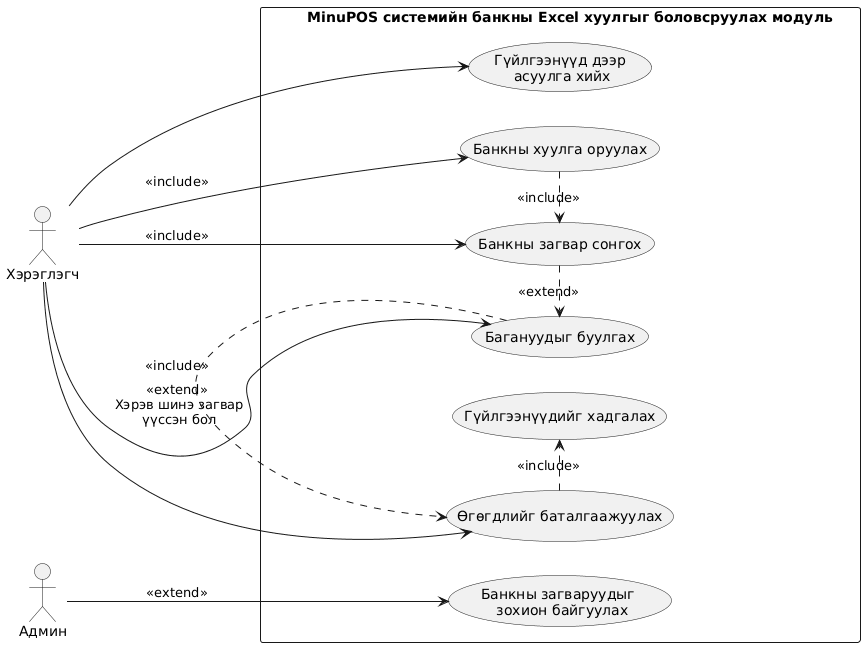
\includegraphics[width=17cm]{images/module_usecase.png}
		\caption{MinuPOS системийн банкны Excel хуулгыг боловсруулах модулийн ажлын явцын диаграм}
		\label{fig:module_usecase}
\end{figure}

Дээрх ажлын явцын диаграмд тусгасан чухал ажлын явцын тайлбаруудыг харгалзах \ref{tab:ucfs01} болон \ref{tab:ucfs02} хүснэгтүүдэд үзүүлэв. Энд ажлын явцын өдөөгч үзэгдэл, тоглогч, угтвар нөхцөл, дараах нөхцөл, үр дүн, тайлбар, өргөтгөл, хувилар болон чанарын шаардлагуудыг тус тус харгалзан үзэв.

%------------------------------------------------------------------------
\begin{longtable}{|L{4cm}|L{\dimexpr\textwidth-4cm-3\tabcolsep-2\arrayrulewidth\relax}|}
\caption{Ажлын явц: Банкны хуулга оруулах (UC-FS-01)}\label{tab:ucfs01}\\ \hline
\textbf{Хэсэг} & \textbf{Агуулга} \\ \hline
\endfirsthead

\multicolumn{2}{c}{\tablename\ \thetable\ -- \textit{үргэлжлэл}} \\ \hline
\textbf{Хэсэг} & \textbf{Агуулга} \\ \hline
\endhead

\hline \multicolumn{2}{r}{\textit{(үргэлжилнэ)}} \\ \hline
\endfoot

\hline
\endlastfoot

Тэмдэглэгээ & UC-FS-01 \\ \hline
Ажлын явцын нэр & Банкны хуулга оруулах \\ \hline
Ангилал & Анхдагч \\ \hline
Тодорхойлолт & Хэрэглэгч нь Монголын 12 банкны аль нэгээс Excel хуулга оруулж, стандарт хэлбэрт шилжүүлэн хадгалах боломжтой. \\ \hline
Өдөөгч үзэгдэл & Хэрэглэгч веб интерфейсээр файл оруулахыг эхлүүлсэн үед \\ \hline
Тоглогч & Банкны хэрэглэгч, Template Mapping үйлчилгээ, Data Validator, PostgreSQL өгөгдлийн сан \\ \hline
Угтвар нөхцөл & 1. Банкны загвар байгаа эсвэл үүсгэж болно.\\ \hline
Дараах нөхцөл & 1. Гүйлгээний мэдээлэл өгөгдлийн санд хадгалагдсан байна.\\
                & 2. Хэрэглэгч үр дүнгийн мэдээлэл авсан байна. \\ \hline
Үр дүн & Стандартчлагдсан санхүүгийн мэдээлэл хэрэглэгчийн атрибутаар хадгалагдсан байна. \\ \hline
Тайлбар & 1. Модуль нь Excel файл болон хэрэглэгчийн сонгосон метадатаг хүлээн авна.\\
              & 2. Метадатагаас банкны төрлийг тодорхойлно.\\
              & 3. Баганын буулгалтын загварыг авна.\\
              & 4. Тохиргооны дүрмээр гүйлгээг задлана.\\
              & 5. Өгөгдлийн бүрэн бүтэн байдал шалгагдана.\\
              & 6. Стандарт $\digamma$ хэлбэрт хөрвүүлнэ.\\
              & 7. Өгөгдлийн санд хадгална.\\ \hline
Өргөтгөл & 3a. Загвар байхгүй тохиолдолд: \\ 
                      & \quad 3a1. Модуль нь баганын буулгалтын загварыг асууна. \\ 
                      & \quad 3a2. Хэрэглэгч талбаруудыг тодорхойлно. \\ 
                      & \quad 3a3. Шинэ загвар үүснэ. \\ 
                      & 5a. Буруу өгөгдөл илэрсэн тохиолдолд: \\ 
                      & \quad 5a1. Хэрэглэгч засаж дахин оруулна. \\ \hline
Онцгой тохиолдол & Өдөөгч: Танигдаагүй файл формат.\\ 
                    & Өдөөгч: Өгөгдлийн сангийн холболт тасарсан.\\ 
                    & Өдөөгч: Засаж болохгүй буруу өгөгдөл. \\ \hline
Чанарын шаардлага & QR-01 (Өгөгдлийн үнэн зөв байдал: 99.9\%)\\ 
          & QR-12 (GDPR нийцтэй байдал)\\ 
          & QR-07 (10,000 бичлэгийг $<$20 секундэд боловсруулна) \\ \hline

\end{longtable}
%------------------------------------------------------------------------
\begin{longtable}{|L{4cm}|L{\dimexpr\textwidth-4cm-3\tabcolsep-2\arrayrulewidth\relax}|}
\caption{Ажлын явц: Банкны загвар үүсгэх (UC-FS-02)}\label{tab:ucfs02}\\ \hline
\textbf{Хэсэг} & \textbf{Агуулга} \\ \hline
\endfirsthead

\multicolumn{2}{c}{\tablename\ \thetable\ -- \textit{үргэлжлэл}} \\ \hline
\textbf{Хэсэг} & \textbf{Агуулга} \\ \hline
\endhead

\hline \multicolumn{2}{r}{\textit{(үргэлжилнэ)}} \\ \hline
\endfoot

\hline
\endlastfoot

Тэмдэглэгээ & UC-FS-02 \\ \hline
Ажлын явцын нэр & Банкны загвар үүсгэх \\ \hline
Ангилал & Анхдагч \\ \hline
Тодорхойлолт & Админ нь шинэ банкны хуулгын форматын баганануудын буулгалтыг тодорхойлж, загвар үүсгэнэ. \\ \hline
Өдөөгч үзэгдэл & Шинэ банк нэмэгдсэн эсвэл форматыг өөрчилсөн тохиолдолд \\ \hline
Тоглогч & Админ \\ \hline
Угтвар нөхцөл & 1. Жишиг хуулга бэлэн байна.\\
               & 2. Стандарт талбарууд тодорхойлогдсон байна. \\ \hline
Дараах нөхцөл & 1. Шинэ загвар хувилбар хадгалагдсан байна.\\ \hline
Үр дүн & Банкны хуулгад ашиглах дахин ашиглах боломжтой буулгалт бүхий загвар үүссэн байна. \\ \hline
Тайлбар & 1. Админ жишиг хуулгыг оруулна.\\
              & 2. Админ багануудыг стандарт талбаруудад буулгана.\\
              & 3. Модуль нь буулгалтын бүрэн бүтэн байдлыг шалгана.\\
              & 4. Загвар хадгалагдана.\\ \hline
Өргөтгөл & 4a. Буулгалт гүйцээгүй тохиолдолд: \\
                      & \quad 4a1. Модуль нь дутагдсан талбаруудыг онцолж харуулна. \\
                      & \quad 4a2. Админ нэмэлт буулгалт оруулна. \\[4pt]
                      & 5a. Өмнөх загвартой зөрчилдөөн гарвал: \\
                      & \quad 5a1. Хувилбаруудын харьцуулалтыг харуулна. \\
                      & \quad 5a2. Админ давхарлах эсэхийг баталгаажуулна. \\ \hline
Онцгой тохиолдол & Өдөөгч: Буруу буулгалтын загвар.\\
                    & Өдөөгч: Хадгалах квота хэтэрсэн. \\ \hline
Чанарын шаардлага & QR-09 (загвар үүсгэх хугацаа $<$ 5 минут)\\
          & QR-14 (Хувилбар зөрчилөөс урьдчилан сэргийлэх)\\ \hline

\end{longtable}


\newpage
\subsection{Функциональ  шаардлага}
Доор MinuPOS системийн банкны Excel хуулгыг боловсруулах модулийн функциональ шаардлагуудыг жагсаав. Дадлага удирдагчийн заавраар хэрэглэгч нэвтрэх/бүртгэх шаардлагыг орхигдуулсан болно. Хэрэглэгч нь админ байж болно.
\begin{table}[h]
\caption{Банкны Excel хуулгыг боловсруулах модулийн функциональ шаардлага}
\begin{tabular}{|p{3cm}|p{13cm}|}
\hline
Шаардлагын нэр & \text{Шаардлагын тайлбар} \\ \hline
ФШ10 & Модуль нь банкны Excel хуулгаас гүйлгээний мэдээллийг (огноо, дүн, тайлбар) уншиж авна. \\ \hline
ФШ11 & Модуль нь өгөгдсөн банкны Excel хуулгаас уншиж авсан мэдээллийг  $\digamma$ стандарт бүтэцтэй объектод хувиргана. $\digamma$ стандарт бүтцийн дэлгэрэнгүйг "Өгөгдлийн бүтэц ба загвар" хэсгээс харна уу. \\ \hline
ФШ12 & Модуль нь өгөгдсөн банкны Excel хуулгын мэдээллийг өгөгдлийн санд хадгалдаг байна. \\ \hline
ФШ13 & Модуль нь хадгалсан гүйлгээнүүд дээр огноо, дүн, тайлбар зэрэг атрибутуудаар хайлт хийх боломжийг олгодог байна. \\ \hline
ФШ20 & Модуль нь хэрэглэгчээс банкны төрлийг оролтоор авдаг байна. \\ \hline
ФШ21 & Модуль нь хэрэглэгчид банкны Excel хуулгын загварыг оролтоор оруулах боломжийг олгодог байна. \\ \hline
ФШ30 & Модуль нь хэрэглэгчээс банкны Excel хуулгыг оролтоор авдаг байна. \\ \hline
ФШ40 & Модуль нь хэрэглэгчид банкны загвар үүсгэх боломжийг олгодог байна. \\ \hline
ФШ41 & Модуль нь хэрэглэгчид хадгалсан банкны загваруудыг засах, устгах боломжийг олгодог байна. \\ \hline
\end{tabular}
\end{table}

\newpage
\subsection{Функциональ бус шаардлага}
\begin{table}[h]
\caption{Банкны Excel хуулгыг боловсруулах модулийн функциональ бус шаардлага}
\begin{tabular}{|p{3cm}|p{13cm}|}
\hline
Шаардлагын нэр & \text{Шаардлагын тайлбар} \\ \hline
ФШБ10 & 1000 хүртэлх мөр бүхий Excel хуулгыг 5 секундын дотор боловсруулж, өгөгдлийн санд амжилттай хадгалдаг байна. \\ \hline
ФБШ20 & Хэрэглэгчийн Excel хуулга оруулах үйлдэл нь ойлгомжтой, 3-аас илүүгүй алхмаар хийгддэг байна. \\ \hline
ФБШ40 & Модуль нь шинэ банкны төрөл эсвэл загварыг нэмэхэд хялбар, үүнийг хийхэд одоо байгаа кодонд их хэмжээний өөрчлөлт хийх шаардлагагүй байна. \\ \hline
ФБШ41 & Код нь цэгцтэй, тайлбар бичигдсэн, өөр хөгжүүлэгч тухайн кодыг ойлгоход хялбар байна. \\ \hline
\end{tabular}
\end{table}

\subsection{Хөгжүүлэлтийн орчинд тавигдах шаардлага}

\begin{table}[h]
\caption{Банкны Excel хуулгыг боловсруулах модулийн хөгжүүлэлтийн орчинд тавигдах шаардлага}
\begin{tabular}{|p{3cm}|p{13cm}|}
\hline
Шаардлагын нэр & \text{Шаардлагын тайлбар} \\ \hline
ХОТШ10 & Модуль хөгжүүлэхэд зориулсан нэгдсэн
хөгжүүлэлтийн орчинг (IDE) ашиглана. \\ \hline
ХОТШ20 & Git зэрэг хувилбарын хяналтын системүүдийг ашигладаг байна. \\ \hline
ХОТШ30 & Өгөгдлийн хадгалахдаа PostgreSQL харьцаат өгөгдлийн санг ашиглана. \\ \hline
\end{tabular}
\end{table}

\newpage
\subsection{Өгөгдлийн бүтэц ба загвар}
Банкны Excel хуулгыг боловсруулах модуль нь $\digamma$ стандарт бүтэцтэй өгөгдлийн загварыг ашиглана. $\digamma$ стандарт бүтэц нь дараах төрөл бүхий талбарыг агуулна:
\subsubsection{Банкны хуулгын өгөгдлийн баганууд}
\begin{table}[h]
\centering
\caption{MinuPOS системийн $\digamma$ стандарт бүтцийн толгой баганууд}
\begin{tabular}{|p{5cm}|p{5cm}|}
\hline
\textbf{Баганы нэр} & \textbf{Өгөгдлийн төрөл} \\ \hline
STATEMENT\_ID & VARCHAR2(20) \\ \hline
REQUEST\_ID & VARCHAR2(20) \\ \hline
BANK\_CODE & VARCHAR2(20) \\ \hline
START\_DATE & DATE \\ \hline
END\_DATE & DATE \\ \hline
TXN\_COUNT & NUMBER \\ \hline
INCOME & NUMBER \\ \hline
OUTCOME & NUMBER \\ \hline
FILE\_ID & VARCHAR2(100) \\ \hline
ACCOUNT\_NO & VARCHAR2(20) \\ \hline
CREATED\_DATE & DATE \\ \hline
STATEMENT\_DATE & DATE \\ \hline
MAIN\_FLAG & VARCHAR2(2) \\ \hline
ACCOUNT\_NAME & VARCHAR2(200) \\ \hline
\end{tabular}
\end{table}
\newpage
\subsubsection{Банкны хуулгын гүйлгээний дэлгэрэнгүй баганууд}
\begin{table}[h]
\centering
\caption{MinuPOS системийн $\digamma$ стандарт бүтцийн дэлгэрэнгүй баганууд}
\begin{tabular}{|p{5cm}|p{5cm}|}
\hline
\textbf{Баганы нэр} & \textbf{Өгөгдлийн төрөл} \\ \hline
DETAIL\_ID & VARCHAR2(20) \\ \hline
STATEMENT\_ID & VARCHAR2(20) \\ \hline
TXN\_DATE & DATE \\ \hline
PRE\_BALANCE & NUMBER \\ \hline
POST\_BALANCE & NUMBER \\ \hline
TXN\_AMOUNT & NUMBER \\ \hline
TXN\_TYPE & VARCHAR2(20) \\ \hline
TXN\_DESC & VARCHAR2(1000) \\ \hline
CO\_ACCOUNT & VARCHAR2(200) \\ \hline
USE\_FLAG & VARCHAR2(2) \\ \hline
USE\_FLAG\_USER\_ID & VARCHAR2(20) \\ \hline
USE\_FLAG\_DATE & DATE \\ \hline
STATUS & VARCHAR2(20) \\ \hline
\end{tabular}
\end{table}

Дадлагын ажлын хүрээнд миний гүйцэтгэх даалгавар нь асуудал шийдэх байсан тул шин- жилгээний үеийн классын диаграмыг үүсгээгүй болно. Гэхдээ статик загварыг доорх зохиом- жийн хэсэгт дэлгэрэнгүй тайлбарлав.

\newpage
\section{MinuPOS системийн банкны Excel хуулгыг боловсруулах модулийн зохиомж}
Энэ хэсэгт MinuPOS системийн банкны Excel хуулгыг боловсруулах модульд ашигласан гол архитектурын үлгэр загваруудыг танилцуулж, тэдгээрийн хэрэглээ, зохиомжийн тайлбарыг өгнө.

\subsection{"Strategy" үлгэр загварын зохиомжийн тайлбар}
Монголын банкууд Excel хуулгаа өөр өөр форматтайгаар өгдөг тул формат бүрт тусдаа, хатуу кодчилсон парсер бичих нь үр ашиггүй. "Strategy" үлгэр загварыг сонгосон гол шалтгаан нь шинэ банк нэмэх, эсвэл хуучин банкны хуулгын формат өөрчлөгдөхөд үндсэн парсингийн логикт өөрчлөлт хийх шаардлагагүй болоход оршино. Зөвхөн шинэ буулгалтын загвар нэмэхэд хангалттай. Ингэснээр код давхардал багасгаж чадна.
% Strategy Pattern-ийг хэрэг- жүүлснээр тухайн банкны Excel хуулгын буулгалтын тохиргоог (JSON хэлбэрээр хадгалсан) ачааллаж, runtime үед сонгосон банкны тохиргоонд тулгуурлан Excel файлыг боловсруулдаг болсон.

\subsection{"Template Method" үлгэр загварын зохиомжийн тайлбар}
Excel хуулга боловсруулахад "Template Method" үлгэр загварыг ашигласан. Ямар ч банкны Excel файлын хувьд ерөнхий алгоритм дараах алхмуудтай ижил байна:

\begin{figure}[h]
		\centering
		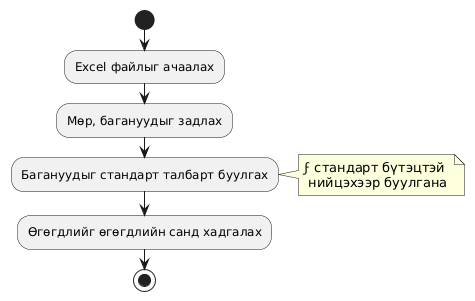
\includegraphics[width=10cm]{images/state.png}
		\caption{Excel хуулга боловсруулах ерөнхий төлөвийн диаграм}
		\label{fig:state}
\end{figure}

Энэ урсгал тогтмол боловч зарим алхам (жишээлбэл, багануудыг хэрхэн буулгах) нь банк бүрийн форматаас хамааран өөрчлөгдөж болно. Үүний тулд бүх хувилбар тус бүрээр дахин код бичихийн оронд ерөнхий алгоритмыг нэг загварт хадгалж, хувьсах алхмуудыг буулгалтын загвараар уян хатан болгож чадна. 

\subsection{"Builder" үлгэр загварын зохиомжийн тайлбар}

Модуль тодорх StatementHdr, StatementDetail зэрэг энтити объектуудыг үүсгэхэд "Builder" үлгэр загварыг ашигласан (\ref{fig:builder} зургийг харна уу). Эдгээр энтитинүүд нь олон талбартай бөгөөд бүх утгууд нь нэг дор бэлэн байдаггүй. Барилгачин нь урт байгуулагч бичихгүйгээр, эсвэл бүх талбарыг гараар тохируулахгүйгээр объектуудыг алхам алхмаар үүсгэх боломжтой болгодог. Ирээдүйд шинэ талбар нэмэх шаардлага гарвал байгуулагч бүрийг өөрчлөхгүй, зөвхөн барилгачинд нэмэхэд хангалттай. (\ref{fig:builder} зургийг харна уу)
\begin{figure}[H]
		\centering
		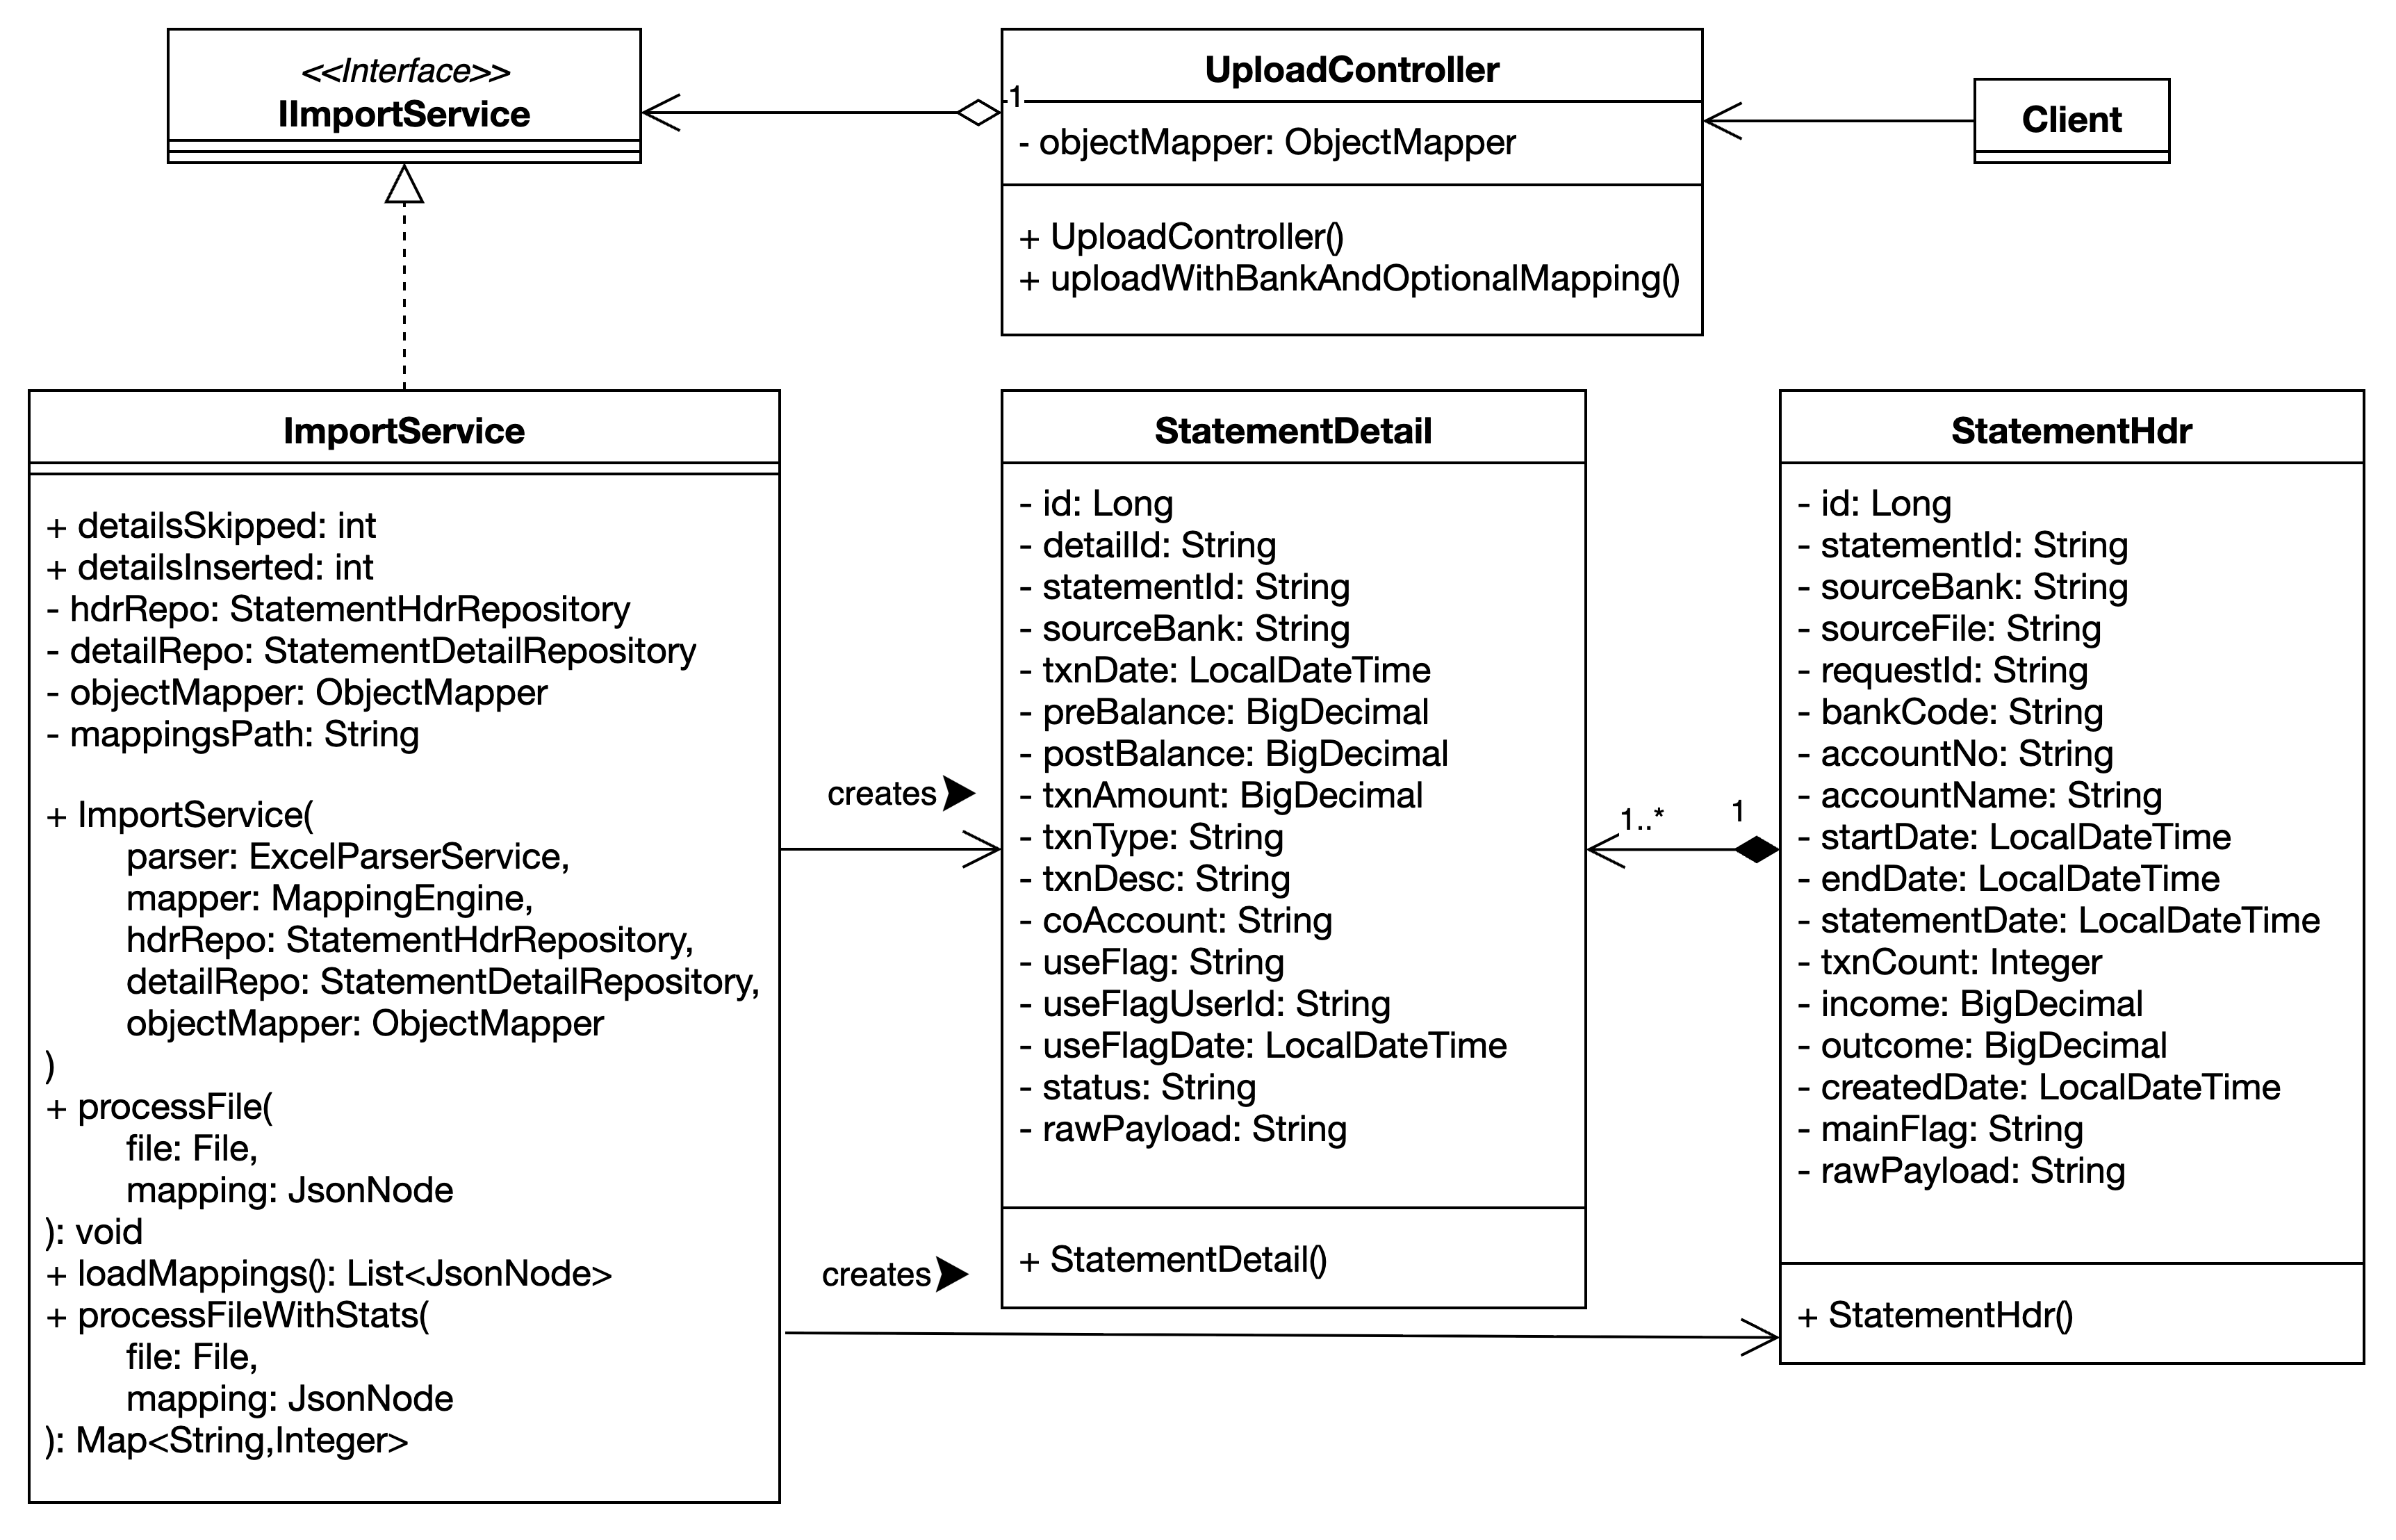
\includegraphics[width=15cm]{images/builder.png}
		\caption{"Builder" үлгэр загварын зохиомжийн диаграм}
		\label{fig:builder}
\end{figure}

\subsection{"Factory" үлгэр загварын зохиомжийн тайлбар}

"Factory" үлгэр загварыг MappingConfigLoader классад тусгасан. Энэ класс нь буулгалтын загвар зэрэг объектуудыг үүсгэх үүрэгтэй бөгөөд тухайн объектыг хэрхэн бүтээх нарийн логикийг системийн бусад хэсэгт ил гаргахгүй. Жишээлбэл, JSON буулгалтын загварыг уншиж, тохирох буулгалтын объект үүсгэх ажлыг хариуцна.

\subsection{Модулийн статик загвар}
Шинжилгээний үед тодорхойлсон өгөгдлийн  $\digamma$ стандарт бүтэцтэй нийцэхээр model багцын классын диаграмыг \ref{fig:model} зурагт үзүүлэв. Мэдээж getter, setter, toString зэрэг агуудыг агуулах бөгөөд эдгээрийг диаграмд оруулаагүй болно. Модулийн гол зохиомжийн диаграмыг \ref{fig:design} зурагт үзүүлэв.

\begin{figure}[H]
		\centering
		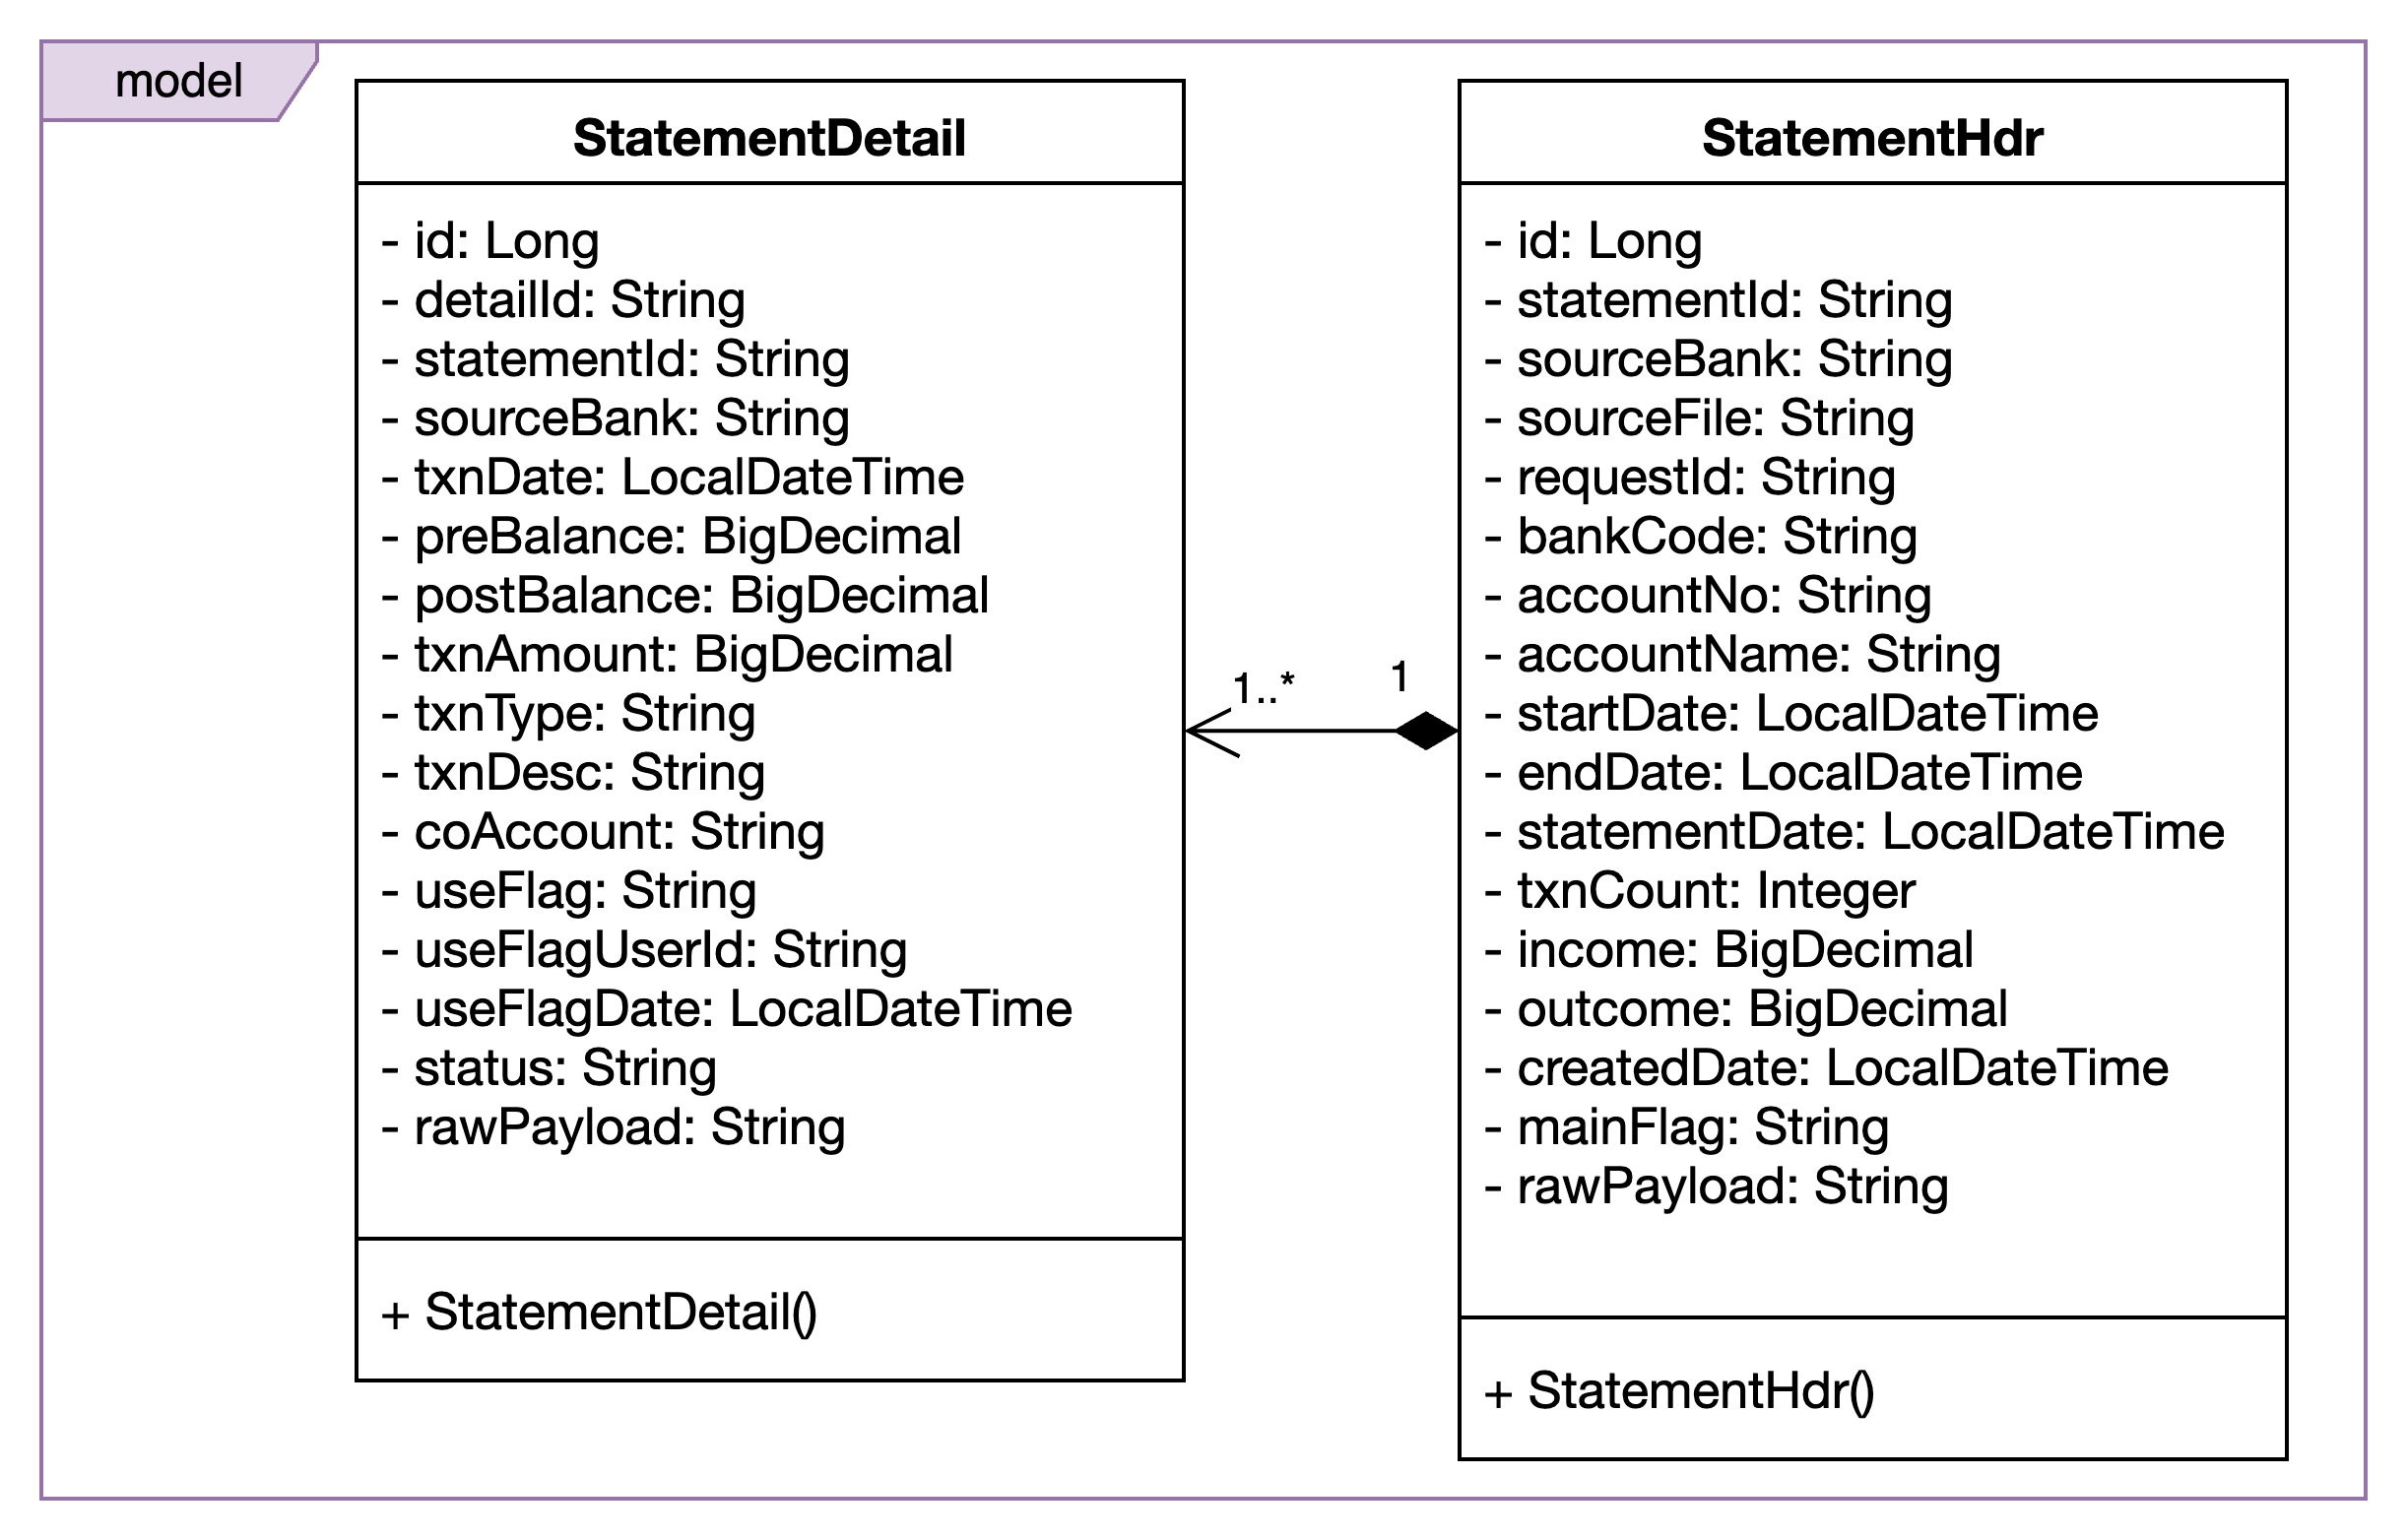
\includegraphics[width=13cm]{images/model.png}
		\caption{MinuPOS системийн банкны Excel хуулгыг боловсруулах модулийн model багцын классын диаграм}
		\label{fig:model}
\end{figure}

\begin{figure}[H]
		\centering
		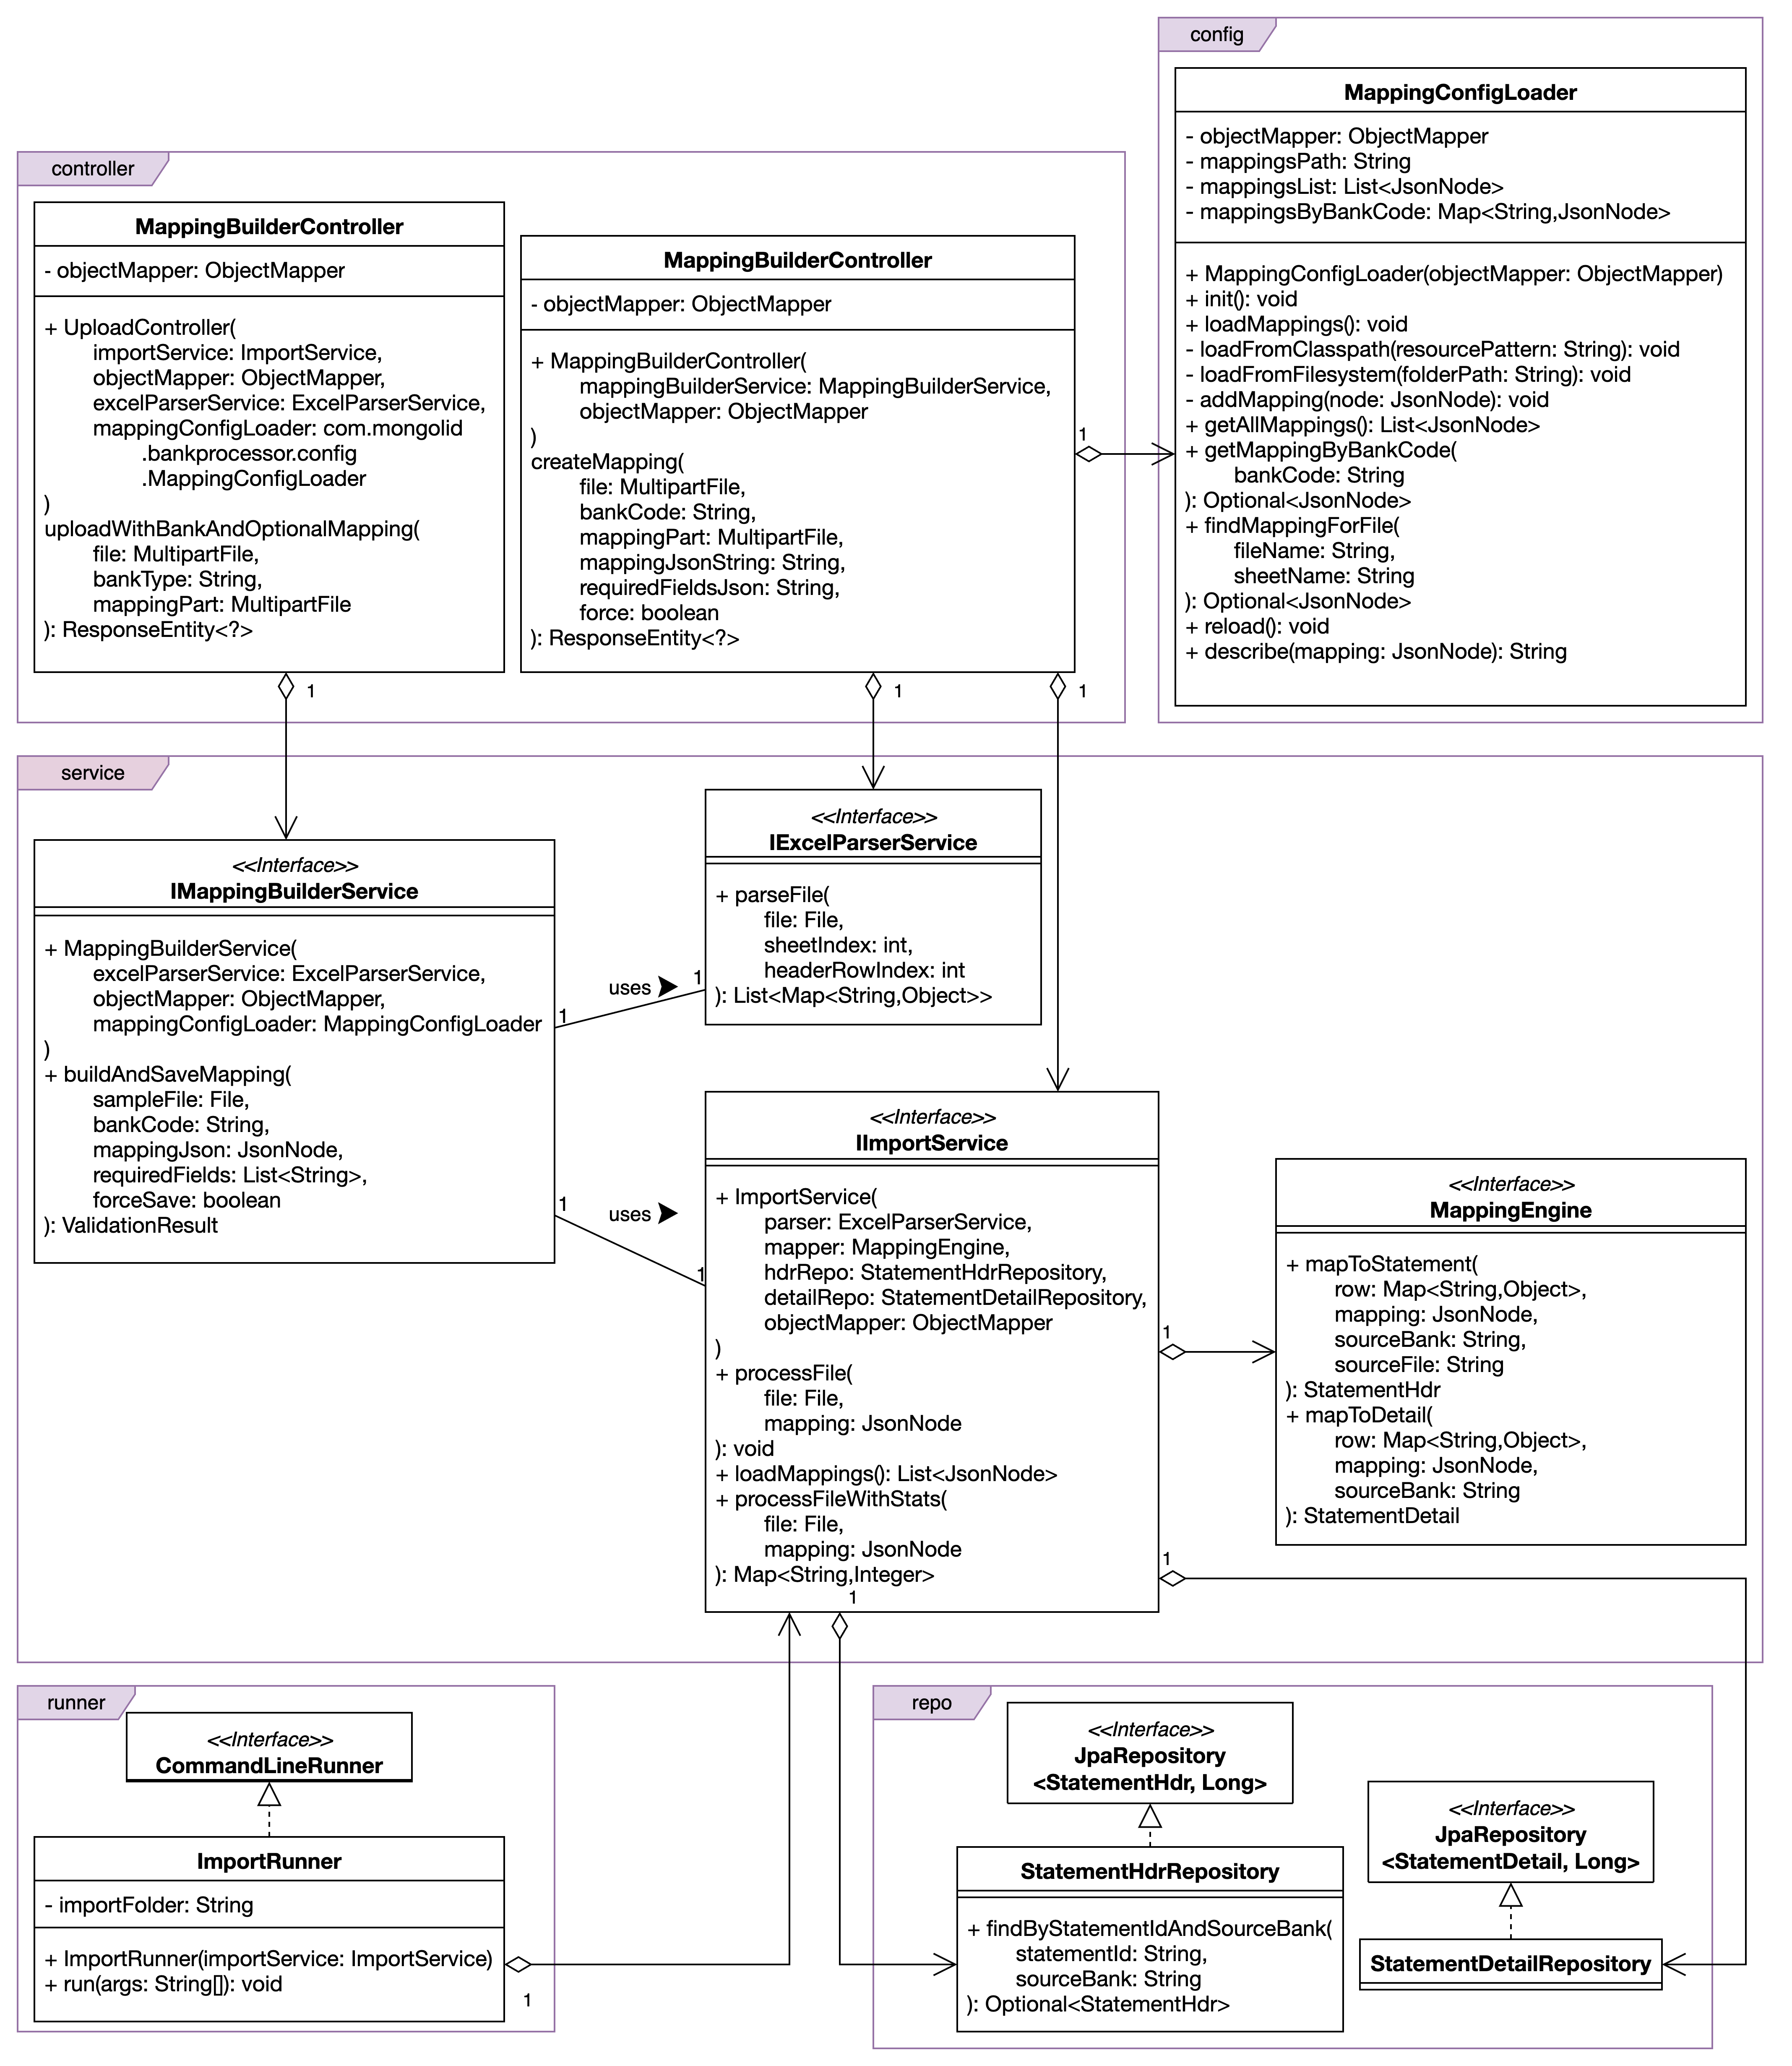
\includegraphics[width=17cm]{images/design.png}
		\caption{MinuPOS системийн банкны Excel хуулгыг боловсруулах модулийн зохиомжийн үеийн классын диаграм}
		\label{fig:design}
\end{figure}

\newpage
\section{MinuPOS системийн банкны Excel хуулгыг боловсруулах модулийн хэрэгжүүлэлт}

\subsection{ExcelParserService}
Файлын форматын олон янз байдлыг дэмжихийн тулд зөвхөн өгөгдсөн буулгалтын загвар дээр тулгуурлан Excel файлаас өгөгдлийг шүүж авдаг байхаар хэрэгжүүлсэн. Жишээлбэл, Excel файлын толгой мөрийн индексийг зааж өгсөн тохиолдолд тухайн мөрөөс баганын нэрсийг задлан, дараагийн мөрүүдийг боловсруулахад ашигладаг. Мөн \verb|FORMULA| төрлийн нүднүүдийн бодит утгыг авах, \verb|NUMERIC| төрлийн нүднүүдийг тоо эсвэл огноо байдлаар ялгаж боловсруулах зэрэгт DataFormatter классыг ашигласан.\\

\quad \quad POI-ийн \verb|"Cannot get a NUMERIC value from a STRING cell"| алдааг засахын тулд CellType-ыг шалгаж, зөвхөн \verb|NUMERIC| үед \verb|getNumericCellValue()| эсвэл \verb|getDateCellValue()| дуудаж, бусад тохиолдолд DataFormatter-аар string утгыг авдаг болгосон. Харин \verb|FORMULA| төрлийн хувьд \verb|getCachedFormulaResultType()| ашиглаж, \verb|row.getLastCellNum()|-ийн давталт дотор \verb|<| нөхцөл тавьсан. Мөн \verb|mapToDetail| болон \verb|mapToStatement| хэсэгт String утгыг Double эсвэл Date рүү parse хийдэг хэсэг нэмсэн.\\
\begin{lstlisting}[language=Java, caption=Excel файлаас DataFormatter ашиглан өгөгдлийг шүүж авах, frame=single]
for (int ci = 0; ci < lastCellNum; ci++) {
		Cell cell = row.getCell(ci);
		String key = headerMap.containsKey(ci) ? headerMap.get(ci) : String.valueOf(ci);
		Object val = null;
		if (cell != null) {
				CellType cellType = cell.getCellType();
				if (cellType == CellType.FORMULA) {
						cellType = cell.getCachedFormulaResultType();
				}

				if (cellType == CellType.NUMERIC) {
						if (DateUtil.isCellDateFormatted(cell)) {
								val = cell.getDateCellValue();
						} else {
								val = cell.getNumericCellValue();
						}
				} else if (cellType == CellType.BOOLEAN) {
						val = cell.getBooleanCellValue();
				} else {
						String txt = dataFormatter.formatCellValue(cell).trim();
						val = txt;
				}

				if (val != null && !(val instanceof String && ((String) val).isEmpty())) {
						allEmpty = false;
				}
		}
		rowMap.put(key, val);
}
\end{lstlisting}


\subsection{ImportService}

ImportService нь Excel файлыг уншиж, буулгалтын загвар ашиглан өгөгдлийг стандарт форматад хувиргаж, өгөгдлийн санд хадгалах гол үйлчилгээ юм. ExcelParserService-ашиглан файлыг задлах, MappingEngine-ээр өгөгдлийг стандарт форматад хувиргах, Repository-гүүдээр өгөгдлийн санд хадгалах, мөн буулгалтын загваруудыг JSON хэлбэрээр нөөцөөс унших зэрэг үүргүүдтэй. Уг үйлчилгээний гол алхмуудыг дараах байдлаар нэгтгэн тайлбарлав:

\begin{itemize}
	\item Буулгалтын загвар байхгүй тохиолдолд файлыг боловсруулахгүй.
	\item Excel-ийн мөрүүдийг \verb|STATEMENT_ID| талбараар ялгаж, толгой өгөгдөл болон дэлгэрэнгүй өгөгдлийг тодорхойлно.
	\item Ижил StatementID-тай өгөгдөл дахин орж ирвэл шинэчлэнэ, эсвэл шинээр үүсгэнэ.
	\item Дэлгэрэнгүй мөрүүдийг холбогдох толгойтой StatementID ашиглан холбоно.
	\item Дутуу эсвэл буруу өгөгдөлтэй мөрүүдийг автоматаар бөглөж, шаардлагатай тохиолдолд алгасаж, алдааны статистикийг цуглуулна.
	\item Нөөцөөс mappings/*.json файлуудыг хайж, бүгдийг уншиж JsonNode объектуудын жагсаалт болгон буцаана.
	\item Импортлох явцад statementsInserted, statementsUpdated, detailsInserted, detailsSkipped зэрэг статистик үзүүлэлтүүдийг цуглуулж, хэрэглэгчдэд үр дүнгийн мэдээлэл өгнө.
\end{itemize}

\begin{lstlisting}[language=Java, caption=Давхардсан өгөгдлийг шийдвэрлэх, frame=single]
	Optional<StatementHdr> existing = (s.getStatementId() != null) ?
					hdrRepo.findByStatementIdAndSourceBank(s.getStatementId(), sourceBank) : Optional.empty();

	if (existing.isPresent()) {
			StatementHdr ex = existing.get();
			ex.setRawPayload(s.getRawPayload());
			ex.setAccountName(s.getAccountName());
			ex.setAccountNo(s.getAccountNo());
			ex.setStartDate(s.getStartDate());
			ex.setEndDate(s.getEndDate());
			hdrRepo.save(ex);
	} else {
			hdrRepo.save(s);
	}
\end{lstlisting}

\begin{lstlisting}[language=Java, caption=Нөөцийн хэсгээс буулгалтын загваруудын мэдээллийг унших, frame=single]
	public List<JsonNode> loadMappings() throws Exception {
			List<JsonNode> list = new ArrayList<>();
			Resource[] resources = new PathMatchingResourcePatternResolver()
							.getResources("classpath*:mappings/*.json");
			for (Resource r : resources) {
					String s;
					try (InputStream in = r.getInputStream()) {
							s = new String(in.readAllBytes(), StandardCharsets.UTF_8);
					}
					if (s != null && !s.isEmpty()) {
							list.add(objectMapper.readTree(s));
					}
			}
			return list;
	}
\end{lstlisting}

\subsection{MappingEngine}

MappingEngine класс нь Excel-ээс уншсан  \verb|Map<String, Object>| хэлбэртэй өгөгдлийг MinuPOS системийн $\digamma$ стандарт бүтэцтэй StatementHdr болон StatementDetail объект руу хувиргах үүрэгтэй. Энэхүү үйлчилгээ нь банк бүрийн Excel хуулгын ялгаатай форматыг уян хатан дэмжих, өгөгдлийн төрөл хувиргалт, гүйлгээний дүнг зөв тодорхойлох, алдааны толерант байдал зэрэг гол асуудлуудыг шийддэг. Уг үйлчилгээний гол алхмуудыг дараах байдлаар нэгтгэн тайлбарлав:
\begin{itemize}
	\item Текст, тоо, огноо зэрэг төрөл бүрийн өгөгдлийг зохих форматад хувиргана.
	\item Банкууд гүйлгээний дүнг \verb|TXN_AMOUNT|, \verb|DEBIT|/\verb|CREDIT|, эсвэл баганын дугаар гэх мэт өөр өөрөөр илэрхийлдэг тул бүх боломжит хэлбэрүүдийг шалгаж, нэгдсэн дүн гаргана.
	\item Excel-ээс уншсан өгөгдлийг тоо, огноо, текст хэлбэрээс стандартчилна.
	\item Excel дотор огноонууд өөр өөр хэлбэрээр хадгалагддаг тул бүх хэлбэрийг стандарт LocalDateTime формат руу хувиргана.
	\item Алдаа гарсан тохиолдолд процесс үргэлжилж, алдаатай өгөгдлийг алгасах боломжтой.
\end{itemize}

MappingEngine болон ImportService-д null-safety хамгаалалт нэмсэн. Ялангуяа mapping, mapping.mapping, statement/detail node-ууд байхгүй үед NPE үүсэхгүй болгов. mapToStatement болон mapToDetail функцүүд null буцааж болох тул ImportService-д үр дүнг шалгаж, null бол хадгалахгүй, алдааны лог бичдэг болгосон. Мөн loadMappings() функц classpath-аас InputStream ашиглан mapping JSON-уудыг зөв уншдаг болсон. Ингэснээр mapping.json дутуу эсвэл буруу үед систем унахгүй, алдааг логлоод үргэлжлүүлдэг болсон.\\ \\ \\
\begin{lstlisting}[language=Java, caption=StatementHdr объект үүсгэх, frame=single]
	public StatementHdr mapToStatement(Map<String, Object> row, JsonNode mapping, String sourceBank, String sourceFile) {
			if (mapping == null || mapping.isMissingNode()) return null;
			JsonNode stmtMap = mapping.get("statement");
			if (stmtMap == null || stmtMap.isNull()) return null;
			StatementHdr s = new StatementHdr();
			s.setSourceBank(sourceBank);
			s.setSourceFile(sourceFile);
			s.setRawPayload(toJson(row));

			s.setStatementId(getString(row, stmtMap, "STATEMENT_ID"));
			s.setRequestId(getString(row, stmtMap, "REQUEST_ID"));
			s.setBankCode(getString(row, stmtMap, "BANK_CODE"));
			s.setAccountNo(getString(row, stmtMap, "ACCOUNT_NO"));
			s.setAccountName(getString(row, stmtMap, "ACCOUNT_NAME"));
			s.setMainFlag(getString(row, stmtMap, "MAIN_FLAG"));
			s.setTxnCount(getInt(row, stmtMap, "TXN_COUNT"));
			s.setIncome(getDecimal(row, stmtMap, "INCOME"));
			s.setOutcome(getDecimal(row, stmtMap, "OUTCOME"));
			s.setStartDate(getDateTime(row, stmtMap, "START_DATE"));
			s.setEndDate(getDateTime(row, stmtMap, "END_DATE"));
			s.setCreatedDate(getDateTime(row, stmtMap, "CREATED_DATE"));
			s.setStatementDate(getDateTime(row, stmtMap, "STATEMENT_DATE"));

			return s;
	}
\end{lstlisting}

\begin{lstlisting}[language=Java, caption=StatementDetail объект үүсгэх, frame=single]
	public StatementDetail mapToDetail(Map<String, Object> row, JsonNode mapping, String sourceBank) {
			if (mapping == null || mapping.isMissingNode()) return null;
			JsonNode dmap = mapping.get("detail");
			if (dmap == null || dmap.isNull()) return null;
			StatementDetail d = new StatementDetail();
			d.setSourceBank(sourceBank);
			d.setRawPayload(toJson(row));

			d.setDetailId(getString(row, dmap, "DETAIL_ID"));
			d.setStatementId(getString(row, dmap, "STATEMENT_ID"));
			d.setTxnType(getString(row, dmap, "TXN_TYPE"));
			d.setTxnDesc(getString(row, dmap, "TXN_DESC"));
			d.setCoAccount(getString(row, dmap, "CO_ACCOUNT"));
			d.setUseFlag(getString(row, dmap, "USE_FLAG"));
			d.setUseFlagUserId(getString(row, dmap, "USE_FLAG_USER_ID"));
			d.setStatus(getString(row, dmap, "STATUS"));

			d.setTxnDate(getDateTime(row, dmap, "TXN_DATE"));
			d.setUseFlagDate(getDateTime(row, dmap, "USE_FLAG_DATE"));

			d.setPreBalance(getDecimal(row, dmap, "PRE_BALANCE"));
			d.setPostBalance(getDecimal(row, dmap, "POST_BALANCE"));
			d.setTxnAmount(pickTxnAmount(row, dmap));
			return d;
	}
\end{lstlisting}

\begin{lstlisting}[language=Java, caption=Өгөгдлийн төрөл хувиргалт, frame=single]
	private String normalizeValue(Object v) {
			if (v == null) return null;
			if (v instanceof Number) {
					double d = ((Number) v).doubleValue();
					if (d == Math.floor(d)) return String.valueOf((long) d);
					return String.valueOf(d);
			} else if (v instanceof Date) {
					return java.time.format.DateTimeFormatter.ISO_LOCAL_DATE_TIME
									.format(((Date) v).toInstant().atZone(ZoneId.systemDefault()).toLocalDateTime());
			} else {
					return String.valueOf(v).trim();
			}
	}
\end{lstlisting}

\begin{lstlisting}[language=Java, caption=Огнооны хувиргалт, frame=single]
	private LocalDateTime getDateTime(Map<String, Object> row, JsonNode mapRoot, String field) {
			try {
					JsonNode node = nodeFor(mapRoot, field);
					if (node == null) return null;
					String key = keyNameFromNode(node);
					if (key == null) return null;
					Object v = row.get(key);
					if (v == null) return null;

					if (v instanceof Date) {
							return LocalDateTime.ofInstant(((Date) v).toInstant(), ZoneId.systemDefault());
					} else if (v instanceof Number) {
							double d = ((Number) v).doubleValue();
							long epochMillis = (long) ((d - 25569d) * 86400d * 1000d); // excel serial -> epoch
							return LocalDateTime.ofInstant(Instant.ofEpochMilli(epochMillis), ZoneId.systemDefault());
					} else {
							String s = String.valueOf(v).trim();
							if (s.isEmpty()) return null;
							try {
									return LocalDateTime.parse(s);
							} catch (Exception e1) {
									try {
											return LocalDate.parse(s).atStartOfDay();
									} catch (Exception e2) {
											try {
													java.time.format.DateTimeFormatter fmt = java.time.format.DateTimeFormatter.ofPattern("yyyy-MM-dd HH:mm:ss");
													return LocalDateTime.parse(s, fmt);
											} catch (Exception e3) {
													// yyyy-MM-dd
													try {
															java.time.format.DateTimeFormatter f2 = java.time.format.DateTimeFormatter.ofPattern("yyyy-MM-dd");
															return LocalDate.parse(s, f2).atStartOfDay();
													} catch (Exception ignore) { }
											}
									}
							}
					}
			} catch (Exception e) {
					// hhe
			}
			return null;
	}
\end{lstlisting}


\subsection{UploadController}

Энэ UploadController класс нь Excel файл болон mapping configuration файлуудыг хүлээн авах, боловсруулах REST API эндпойнтуудыг нэгтгэсэн Spring Boot контроллер юм. Үндсэн үүргүүд нь:
\begin{itemize}
	\item Excel файлыг Multipart form data хэлбэрээр хүлээн авах.
	\item Хэрэглэгчийн өгсөн эсвэл системд бэлэн байгаа буулгалтыг ашиглаж буулгалтын загвар боловсруулах.
	\item ImportService-ийг дуудаж импортлох үйл явцыг эхлүүлэх.
	\item Импортын статистик мэдээлэлтэй хамт үр дүнг буцаах.
\end{itemize}

\begin{lstlisting}[language=Java, caption=Буулгалтын загвар боловсруулах, frame=single]
JsonNode mappingJson = null;
if (mappingPart != null && !mappingPart.isEmpty()) {
	tempMappingPath = Files.createTempFile("mapping-", ".json");
	mappingPart.transferTo(tempMappingPath.toFile());
	String mappingContent = Files.readString(tempMappingPath);
	mappingJson = objectMapper.readTree(mappingContent);
	logger.info("Using user-supplied mapping (mapping file).");
} else {
	Optional<JsonNode> maybe = mappingConfigLoader.getMappingByBankCode(bankType);
	if (maybe.isPresent()) {
		mappingJson = maybe.get();
		logger.info("Using mapping from MappingConfigLoader for bankType={}", bankType);
	} else {
		return ResponseEntity.badRequest().body(Map.of(
				"error", "No mapping provided and no mapping found for bankType: " + bankType,
				"hint", "Upload a mapping JSON with the multipart key 'mapping' or add a mapping file to mappings/ folder"
		));
	}
}
\end{lstlisting}
Хэрэглэгч буулгалтын файл өгсөн бол түүнийг, үгүй бол системийн буулгалтын загварыг ашиглана.

\begin{lstlisting}[language=Java, caption=БФайлын урьдчилсан харагдац үүсгэх, frame=single]
int sheetIndex = mappingJson.path("sheet").asInt(0);
int headerRowIndex = mappingJson.path("headerRowIndex").asInt(-1);
var previewRows = excelParserService.parseFile(tempFilePath.toFile(), sheetIndex, headerRowIndex);
int previewCount = previewRows.size();
\end{lstlisting}

\subsection{MappingConfigLoader}
MappingConfigLoader классыг хэрэгжүүлэхэд банк бүрийн Excel хуулгын формат, файл нэр, sheet нэр, баганын бүтэц зэрэг маш олон янзын хувилбарыг уян хатан дэмжих шаардлагыг голчлон анхаарсан. Өмнө нь формат бүрт тусдаа парсер, код бичих шаардлагатай байсан нь засварлахад хүндрэлтэй, алдааны магадлал өндөр байв. Иймд дараах зарчмуудыг баримталсан:

\begin{itemize}
	\item MappingConfigLoader нь буулгалт JSON-уудыг classpath-аас болон файл системээс ачаалах боломжтой. Ингэснээр deployment бүрт тохиргооны файлуудыг өөрчлөх, шинэ банк нэмэхэд кодонд өөрчлөлт хийхгүйгээр шийдэж чадна.
	\item Банк бүрийн буулгалтыг bankCode-оор индексжүүлж, хурдан lookup хийх боломжтой болгосон. Энэ нь олон буулгалт дундаас зөв буулгалтыг автоматаар сонгоход чухал.
	\item Файлын нэрээр буулгалтыг автоматаар олж сонгох логик нэмсэн. Ингэснээр хэрэглэгч буруу буулгалт сонгох эрсдэл багассан.
	\item Буулгалтуудыг runtime үед дахин ачаалах боломжтой болгосон. Энэ нь production орчинд шинэ буулгалт нэмэх, засварлахад системийг зогсоохгүйгээр шийдэж чадна.
	\item Буулгалтын файл буруу, дутуу, эсвэл parse алдаа гарсан тохиолдолд бусад буулгалтуудыг үргэлжлүүлэн ачаалж, системийн үндсэн үйл ажиллагаа тасалдахгүй байхаар шийдсэн.
\end{itemize}

Эдгээр шийдлүүдийн үр дүнд MinuPOS системд шинэ банк нэмэх, хуучин банкны формат өөрчлөгдөх, буулгалт-ийг засварлах зэрэг бүх үйлдлийг кодонд өөрчлөлт хийхгүйгээр зөвхөн буулгалт JSON-уудыг засах замаар шийддэг болсон. Энэ нь хөгжүүлэлтийн хурд, засварлахад хялбар байдал, алдааны магадлалыг эрс бууруулсан.

\begin{lstlisting}[language=Java, frame=single, caption=Classpath-аас буулгалтын JSON-уудыг ачаалах]
private void loadFromClasspath(String resourcePattern) {
		try {
				logger.info("Loading mapping resources from classpath pattern '{}'", resourcePattern);
				PathMatchingResourcePatternResolver resolver = new PathMatchingResourcePatternResolver();
				Resource[] resources = resolver.getResources(resourcePattern);
				for (Resource r : resources) {
						try {
								JsonNode node = objectMapper.readTree(r.getInputStream());
								addMapping(node);
								logger.debug("Loaded mapping from classpath resource: {}", r.getFilename());
						} catch (Exception e) {
								logger.warn("Failed to parse mapping resource {}: {}", r.getFilename(), e.getMessage());
						}
				}
		} catch (IOException e) {
				logger.warn("No mapping resources found for pattern {}: {}", resourcePattern, e.getMessage());
		}
}
\end{lstlisting}

\begin{lstlisting}[language=Java, frame=single, caption=Файл системээс mapping JSON-уудыг ачаалах]
private void loadFromFilesystem(String folderPath) {
		File folder = new File(folderPath);
		if (!folder.exists() || !folder.isDirectory()) {
				logger.debug("Mappings folder '{}' does not exist or not a directory — skipping filesystem load.", folderPath);
				return;
		}
		logger.info("Loading mapping JSON files from filesystem folder '{}'", folderPath);
		File[] files = folder.listFiles((d, name) -> name.toLowerCase().endsWith(".json"));
		if (files == null) return;
		Arrays.stream(files).sorted().forEach(f -> {
				try {
						String content = new String(Files.readAllBytes(f.toPath()));
						JsonNode node = objectMapper.readTree(content);
						addMapping(node);
						logger.debug("Loaded mapping from filesystem file: {}", f.getName());
				} catch (Exception e) {
						logger.warn("Failed to parse mapping file {}: {}", f.getName(), e.getMessage());
				}
		});
}
\end{lstlisting}

\begin{lstlisting}[language=Java, frame=single, caption=Банкны кодоор mapping-ийг индексжүүлэх]
private void addMapping(JsonNode node) {
	mappingsList.add(node);
	
	JsonNode bankCodeNode = node.get("bankCode");
	if (bankCodeNode != null && bankCodeNode.isTextual()) {
		String bankCode = bankCodeNode.asText().trim();
		if (!bankCode.isEmpty()) {
			mappingsByBankCode.put(bankCode, node);
		}
	}
}
\end{lstlisting}

\begin{lstlisting}[language=Java, frame=single, caption=Файлын нэрээр mapping автоматаар сонгох]
public Optional<JsonNode> findMappingForFile(String fileName, String sheetName) {
		if (fileName == null) return Optional.empty();
		String name = new File(fileName).getName();
		// 1
		for (JsonNode cfg : mappingsList) {
				JsonNode patterns = cfg.get("filePatterns");
				if (patterns != null && patterns.isArray()) {
						for (JsonNode p : patterns) {
								if (!p.isTextual()) continue;
								String patternText = p.asText().trim();
								if (patternText.isEmpty()) continue;

								try {
										Pattern pattern = Pattern.compile(patternText);
										if (pattern.matcher(name).find()) {
												return Optional.of(cfg);
										}
								} catch (Exception rex) {matching (strip .* common pattern)
										String plain = patternText.replace(".*", "");
										if (!plain.isEmpty() && name.contains(plain)) {
												return Optional.of(cfg);
										}
								}
						}
				}
		}

		// 2
		if (sheetName != null && !sheetName.trim().isEmpty()) {
				String sheet = sheetName.trim().toLowerCase();
				for (JsonNode cfg : mappingsList) {
						JsonNode sheetNode = cfg.get("sheetName");
						if (sheetNode != null && sheetNode.isTextual()) {
								String s = sheetNode.asText().trim().toLowerCase();
								if (!s.isEmpty() && sheet.contains(s)) {
										return Optional.of(cfg);
								}
						}
				}
		}
		// 3
		if (mappingsList.size() == 1) {
				return Optional.of(mappingsList.get(0));
		}
		return Optional.empty();
}
\end{lstlisting}

\begin{lstlisting}[language=Java, frame=single, caption=Runtime reload хийх capability]
public synchronized void reload() {
	try {
		loadMappings();
	} catch (IOException e) {
		logger.error("Failed to reload mapping files: {}", e.getMessage(), e);
	}
}
\end{lstlisting}
